\section{Inspector-Executor}

In its non-blocking mode of execution, GraphBLAS allows specific implementations to support
various alternative execution approaches. In particular, it allows for non-terminating methods to be 
executed in several stages, possibly interleaved with stages from other methods. This is called \emph{split execution}. In a particular split execution,
a method can go through an \emph{analyze} stage followed by a \emph{perform} stage.
The analyze stage computes various characteristics of the object being produced, whereas the
perform stage does the actual calculations.

It may be desirable to augment GraphBLAS with additional constructs to control this particular
analyze/perform split explicitly. In particular, having the application communicate properties of
an object that do not change between multiple perform stages, and therefore greatly simplifies
or eliminates the need for analyze stages, could be valuable.

As a concrete example, the current GraphBLAS specification exposes {\sf mxm} as a single operation to the user. Under the hood, it is understood that {\sf mxm} is typically implemented in two phases: analyze and compute. The analyze phase consists of allocating memory to the output matrix. The compute phase computes the value at each nonzero of the output matrix. The implementer has the option of deciding whether to set the nonzero structure of the output matrix in the analyze phase or the compute phase.

It may be desirable in some circumstances to expose these two phases of {\sf mxm} to the user as {\sf mxm\_analyze} and {\sf mxm\_compute}. 

For typical use cases, both the size and nonzero structure of the output matrix \textbf{C} is not known \emph{a priori} before the {\sf mxm} operation is run. However, there may exist situations where the user is computing a sequence of output matrices \textbf{C} for which the output nonzeroes share the same \emph{structural zeroes} and therefore, memory allocation. In this case, it may be advantageous for the user to call {\sf mxm\_analyze} and {\sf mxm\_compute} for the first matrix-multiplication in the sequence, and {\sf mxm\_compute} for the rest.

We used two experimental testbeds to test the importance of \emph{split execution} for {\sf mxm} operation. Experiments were performed on a quad-core Intel Xeon CPU E5-2637 v2 @ 3.50GHz with 256 GB RAM running Ubuntu 14.04.1, and an NVIDIA K40c GPU with 12 GB RAM. Some more details of the test setups are listed in Table~\ref{Tab:testbed}.

For our datasets (see Table~\ref{Tab:testset}), we chose six matrices from the University of Florida Sparse Matrix Collection~\cite{davis2011university} because they come from diverse sources (epidemic modeling, finite element modeling, protein data, web connectivity) and have varying sparsity structures ranging from fairly regular (\emph{epidemiology}, \emph{wind tunnel}, \emph{protein}, \emph{sphere}) to highly irregular (\emph{hood}, \emph{webbase}). To test the above mentioned use case, we compared calling {\sf mxm} ten times with no split execution, to a split execution where a call to {\sf mxm\_analyze} is followed by ten calls to {\sf mxm\_compute}.

From Figure~\ref{Fig:gflops}, one immediately sees that the split execution performs better than the unsplit execution. MKL sees a geomean 37.2\% speedup going to split execution, while cuSPARSE sees a geomean 29.3\% speedup. In general, cuSPARSE performed better than MKL on the larger datasets (\emph{wind tunnel}, \emph{protein} and \emph{sphere}), but worse on the smaller ones (\emph{epidemiology} and \emph{webbase}.

\begin{table}[htb]
	\hrule
	\caption{Experimental setup used for benchmarking.}
	\label{Tab:testbed}
	\begin{center}
		\begin{tabular}{|c|c|c|} \hline
			Vendor & Intel & Nvidia \\ \hline
			Family & Xeon & Tesla GPU \\
			Device & E5-2637 v2 & K40c \\
			Codename & Sandy Bridge & Kepler GK110 \\
			Memory & 256 GB & 12 GB \\
			OS & Ubuntu 14.04.1 & Ubuntu 14.04.1 \\
			Compiler & Intel C++ v17.0.4 & nvcc v8.0.44 \\
			& Intel OpenMP v5.0 & g++ v4.9.4 \\
			Library & Intel MKL 2017.4.196 & cuSPARSE v8.0.44 \\ 
			API & mkl\_Scsrmultcsr & cusparseScsrgemm2 \\ \hline
		\end{tabular}
	\end{center}
	\hrule
\end{table}

\begin{table}[htb]
	\hrule
	\caption{Description of datasets used for benchmarking. Flops refers to the number of floating-point computations required to square the matrix by itself. Two copies of the matrix are kept in memory for sake of benchmarking.}
	\label{Tab:testset}
	\begin{center}
		\begin{tabular}{|c|c|c|c|c|} \hline
			Dataset & Rows & Nonzeros & Flops & Symmetric\\ \hline
			\emph{epidemiology} & 526k & 2.1M & 16.8M & no \\
			\emph{wind tunnel} & 218k & 11.6M & 1.3B & yes \\
			\emph{protein} & 36k & 4.3M & 1.1B & yes\\
			\emph{sphere} & 83k & 6.0M & 0.9B & yes\\
			\emph{hood} & 221k & 10.8M & 1.1B & yes \\
			\emph{webbase} & 1.0M & 3.1M & 139M & no \\ \hline
		\end{tabular}
	\end{center}
	\hrule
\end{table}

\begin{figure}
	\centering
	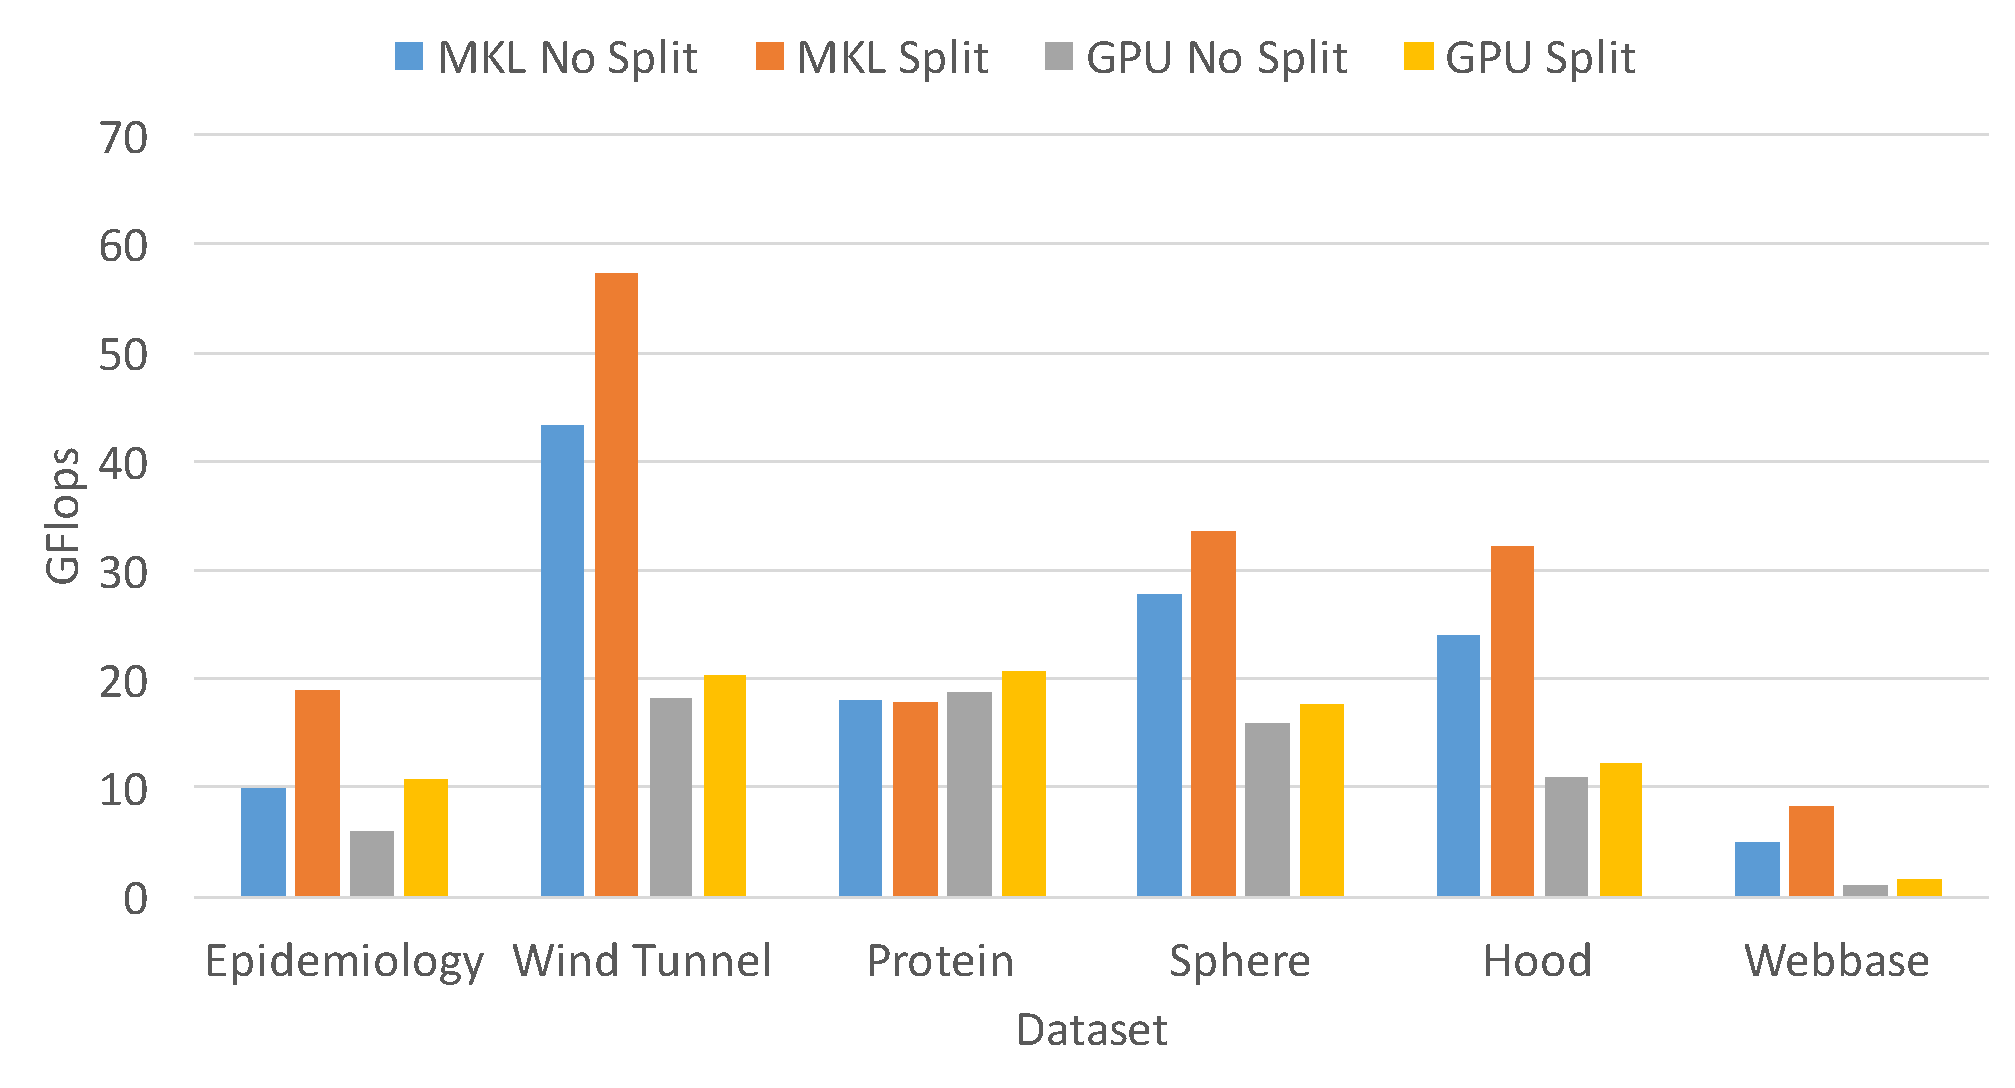
\includegraphics[width=.9\linewidth]{gflops.pdf}
	\caption{Comparison of {\sf mxm} runtime with and without split execution for two experimental setups, MKL and cuSPARSE.}
	\label{Fig:gflops}
\end{figure}

We decided to defer such facilities from version 1.0 of the GraphBLAS specification. There is a computational benefit to the user in being able to access split execution, but the API will need to become more complex in order to support it. We believe that additional experience with implementation and use of GraphBLAS is necessary before we can define the proper interfaces for explicit split execution.